\chapter{Introduzione alla sicurezza di rete}

\section{Firewall e IDS}

Innanzi definiamo che cos'è un \textit{Firewall}

\dfn{Firewall}{
        Si definisce \textbf{Firewall} un sistema di sicurezza che isola una rete interna di un'organizzazione da internet, controllando e filtrando il traffico di rete in entrata e uscita in base a regole di sicurezza definite dette di \texttt{ACCESS} o \texttt{DENIED}
}

L'idea del Firewall è che l'esterno di una rete è composta dai cosiddetti "cattivi ragazzi" che la mamma non vi raccomanderebbe come compagni d'uscita, mentre l'interno della rete è composta da "bravi ragazzi" di cui fidarsi, lo scopo del sistema è, quindi, separare i buoni dai cattivi

\begin{center}
    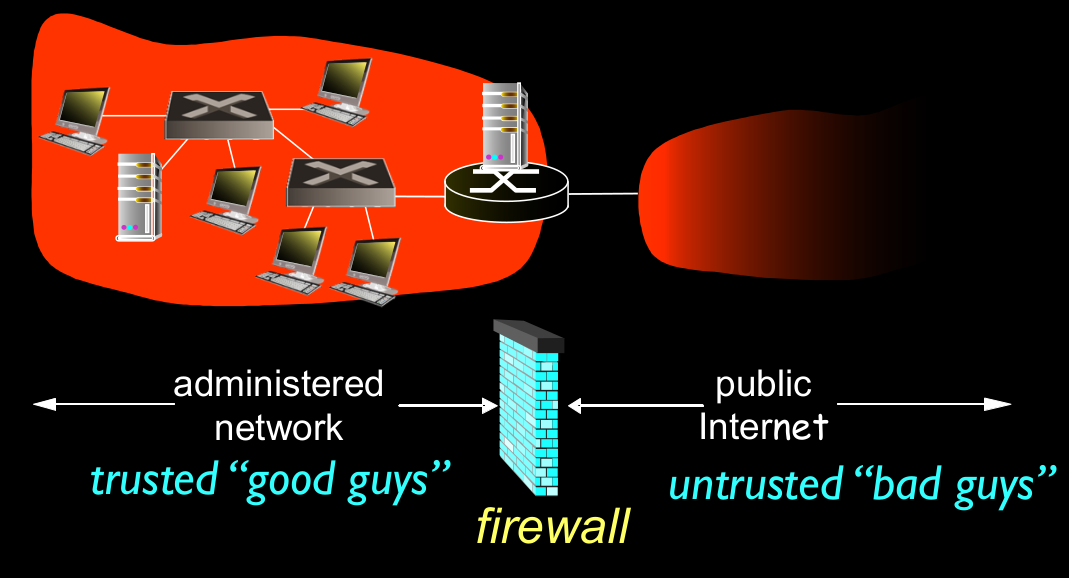
\includegraphics[width=10cm]{img/buoni_cattivi_e_firewall.png}
\end{center}

Il Firewall si rivela utile per principalmente tre motivi:
\begin{itemize}
    \item \textbf{Prevenzione degli attacchi Denial of Service (Dos)}: tipologia di attacco informatico che mira a rendere inaccessibili o indisponibili i servizi di una rete ad utenti legittimi
    
    Un esempio è il \textbf{SYN flooding} in cui un attaccante invia molte richieste di connessione false, esaurendo le risorse del server sovraccaricandolo e impedendo connessioni legittime

    \item \textbf{Protezione dei dati interni da accessi non autorizzati}: ovvero impedisce che gli attaccanti possona \textit{modificare o rubare dati sensibili}
    
    Un esempio classico è un attaccante che sostituisce il sito web di un'organizzazione con un contenuto malevolo.

    \item \textbf{Accesso selettivo e autorizzato alla rete interna}: Permette l’accesso solo a utenti o dispositivi autenticati, migliorando la sicurezza
\end{itemize}

Esistono tre tipi di tipoligie di Firewall che approfonoidremo nel dettaglio:
\begin{itemize}
    \item \textbf{Stateless Packet Filter}: Controlla ogni pacchetto singolarmente, senza tenere traccia delle connessioni
    \item \textbf{Statefull Packet Filter}: Tiene traccia dello stato delle connessioni (es. richieste e risposte)  
    \item \textbf{Application Gateway} (proxy Firewall): controlla il traffico a livello applicativo (es. HTTP, FTP, e.mail), filtrando così le informazioni che all'interno dei protocolli del livello (ad esempio il contenuto di una mail)
\end{itemize}

Si notino nel dettaglio
\subsection{Stateless Packet Filtering}

\dfn{Stateless Packet Filtering}{
    Lo \textbf{Stateless Packet Filtering} è una tecnica di sicurezza di rete in cui un firewall esamina ogni pacchetto individualmente, senza tener conto delle connessioni stabilite in precedenza. Questo significa che ogni pacchetto è valutato isolatamente sulla base di un insieme di regole predefinite
}
Di solito un firewall con filtraggio stateless è implementato su un router che collega una rete interna a internet. Il router analizza ogni pacchetto in ingresso e in uscita e decide se bloccarlo o lasciarlo in base a regole definite nelle cosiddette "\textbf{white list}" (pacchetti che possono passare) e o "\textbf{black list}" (lista di pacchetti da bloccare)

Il firewall prende decisioni basandosi su parametri del pacchetto, tra cui:
\begin{itemize}
    \item \textbf{IP} del mittente e destinatario
    \item \textbf{Numero di porta TCP/UDP} del mittente e destinatario
    \item \textbf{Tipo di messaggio ICMP} bloccando, ad esempio, attacchi di scansione provenienti dall'esterno
    \item \textbf{bit SYN e ACK nei pacchetti TCP}: Il firewall può, ad esempio, bloccare pacchetti con SYN in entrata per impedire connessioni indesiderate dall'esterno
\end{itemize}

Qui degli esempietti:
\ex{Bloccare tutti i pacchetti con protocollo UDP o Telnet}{
    \begin{itemize}
        \item \textbf{Regola}: blocca i pacchetti in entrata e in uscita se il protocollo IP è 17 (UDP) e se con la porta di origine o desitinazione è 23
        \item \textbf{Risultato}: Tutto il traffico UDP  e telnet vengono bloccati
    \end{itemize}
}

\ex{Bloccare pacchetti TCP in ingresso con ACK=0}{
    \begin{itemize}
        \item \textbf{Regola}: blocca tutti i pacchetti TCP in ingresso se il bit ACK = 0
        \item \textbf{Risultato}:Le connessioni in entrata non possono essere iniziate da un host esterno verso la rete interna e le connessioni in uscita funzionano normalmente, perché il traffico di ritorno (che ha ACK=1) è consentito.
    \end{itemize}
}

Riporto qui una tabella con altri esempi:
\begin{center}
    \begin{tabularx}{\textwidth}{|X|X|}
        \hline
        \textbf{Politica} & \textbf{Impostazione Firewall} \\
        \hline
        Nessun accesso Web esterno. & Elimina tutti i pacchetti in uscita verso qualsiasi indirizzo IP, porta 80 \\
        \hline
        Nessuna connessione TCP in entrata, tranne quelle per il server Web pubblico dell'istituzione. & Elimina tutti i pacchetti TCP SYN in entrata verso qualsiasi IP tranne 130.207.244.203, porta 80 \\
        \hline
        Impedisci alle Web-radio di consumare la larghezza di banda disponibile. & Elimina tutti i pacchetti UDP in entrata - tranne DNS e broadcast del router. \\
        \hline
        Impedisci alla tua rete di essere utilizzata per un attacco DoS smurf. & Elimina tutti i pacchetti ICMP diretti a un indirizzo di “broadcast” (ad esempio, 130.207.255.255). \\
        \hline
        Impedisci alla tua rete di essere tracciata & Elimina tutto il traffico ICMP TTL scaduto in uscita \\
        \hline
        \end{tabularx}
\end{center}

\subsubsection{Access control list}
\dfn{Liste di controllo d'accesso}{
    Le \textbf{ACL} sono tabelle di regole applicate, \textit{con priorità dall'alto verso il basso}, ai pacchetti in arrivo per decidere se consentire (allow) o bloccare (deny) il traffico di rete
}

Queste tabelle sono il vero e proprio cuore pulsante del Firewall e indicano quale pacchetto può passare e chi no
\ex{ACL}{
    \begin{center}
        \begin{tabularx}{0.5\textwidth}{|l|l|l|l|l|l|l|}
            \hline
            \textbf{azione} & \textbf{indirizzo sorgente} & \textbf{indirizzo destinazione} & \textbf{protocollo} & \textbf{porta sorgente} & \textbf{porta destinazione} & \textbf{flag bit} \\
            \hline
            allow & 222.22/16 & outside of 222.22/16 & TCP & $>$ 1023 & 80 & any \\
            \hline
            allow & outside of 222.22/16 & 222.22/16 & TCP & 80 & $>$ 1023 & ACK \\
            \hline
            allow & 222.22/16 & outside of 222.22/16 & UDP & $>$ 1023 & 53 & --- \\
            \hline
            allow & outside of 222.22/16 & 222.22/16 & UDP & 53 & $>$ 1023 & --- \\
            \hline
            deny & all & all & all & all & all & all \\
            \hline
        \end{tabularx}
            
    \end{center}
}
\subsubsection{Criticità}
Un serio problema dei Firewall Stateless che potrebbero lasciare passare pacchetti che non hanno senso nel contesto di una connessione.
Esempio:
\begin{itemize}
    \item Un pacchetto con destinazione porta 80 (HTTP) e ACK=1 arriva dall'esterno
    \item Il firewall stateless lo accetta, anche se nessuna connessione HTTP è stata avviata da un client interno.
    \item Un attaccante potrebbe sfruttare questa debolezza per inviare pacchetti falsi alla rete interna
\end{itemize}

Per porre rimedio a questi tipi di problemi si veda la tipoligia di firewall sucessiva

\subsection{Stateful packet filtering}
\dfn{Stateful packet filtering}{
    Lo \textbf{Stateful packet filtering} è una tecnica di filtraggio di pacchetti tenendo traccia delle connessioni attive e delle loro fasi
}
Un firewall stateful tiene traccia di ogni connessione TCP attiva e controlla le tre fasi fondamentali della connessione TCP (assicurandosi che ogni pacchetto in entrata o uscita abbia senso):
\begin{itemize}
    \item \textbf{Setup}: Il firewall rileva il pacchetto SYN iniziale, segnalando l'inizio di una connessione
    \item \textbf{Trasferimento dati}: I pacchetti con ACK vengono accettati solo se appartengono a una connessione già avviata
    \item \textbf{Chiusura}: Quando un pacchetto FIN o un timeout segna la fine di una connessione, il firewall non accetta più pacchetti fino a che non se apre un altro
\end{itemize} 

